\documentclass[a4paper, 11pt]{article}
\usepackage[english]{babel}
\usepackage[T1]{fontenc}
\usepackage[utf8]{inputenc}

% Import images from media folder.
\usepackage{graphicx}
\graphicspath{ {./media/} }

% Header & Footer
% \usepackage{fancyhdr}
% \pagestyle{fancy}
% \lhead{Konrad M. L. Claesson}

\usepackage{soul, color} % Strikethrough, highlight
\usepackage{enumitem} % Enumerate using letters, a) b) c), ...

% No default paragraph indentation.
\setlength{\parindent}{0px}
\renewcommand{\baselinestretch}{1.325}

% Change Paragraph Spacing
\usepackage{setspace}

% Double quotes, \say{}.
\usepackage{dirtytalk}

% Block quotes
\usepackage{etoolbox}
\AtBeginEnvironment{quote}{\singlespacing\small}

% Title
\title{Natural Deduction Proof Verifier} 
\author{Konrad M. L. Claesson\\ konradcl@kth.se\\ 
Lab 2 $-$ DD1351}
\date{\today}

\begin{document}
   \maketitle

   \section{Introduction}
   Natural deduction is a proof calculus comprised of a set of
   inference rules that are used to infer formulas from other
   formulas. The rules can be categorized into introduction
   and elimination rules. The former combine or negate
   formulas by introducing connectives; the latter decompose
   them by eliminating connectives. These rules are defined in
   terms of formula patterns that must hold true for a 
   connective to be introduced or eliminated. For instance, to
   claim $\phi \wedge \psi$, it must be known that
   both of the formulas $\phi$ and $\psi$ are true. Prolog is
   a logic programming language that enables easy expression 
   of logical statements. To exemplify, the Prolog code
   
\begin{verbatim}
   rule(_, [_, and(X, Y), andint(R1, R2)], Verified) :-
      member([R1, X, _], Verified),
      member([R2, Y, _], Verified).
\end{verbatim}
   
   states that $\phi \wedge \psi$ can be concluded, by the and
   introduction rule, if both $\phi$ and $\psi$ are known to
   be true. 
   \bigbreak

   This report presents a Prolog-based algorithm that can
   verify the validity of any proof in propositional logical 
   that has been written exclusively using the rules of
   natural deduction listed in the below table.

   \begin{figure}
      \centering
      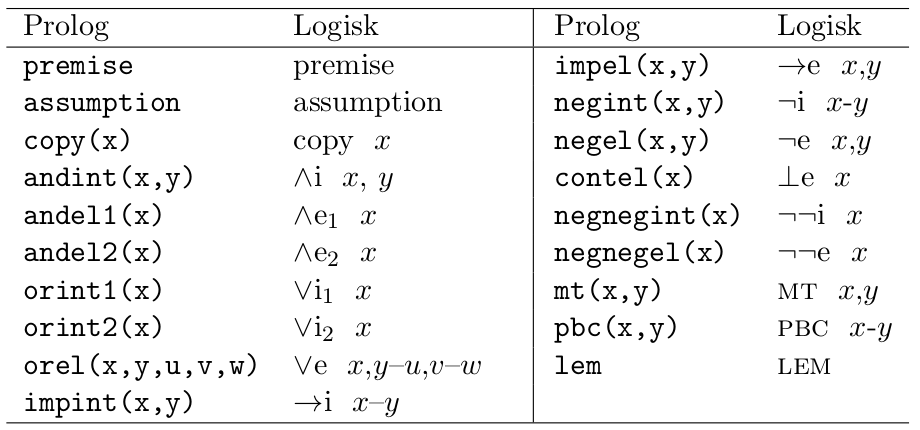
\includegraphics[scale=0.325]{inference-rules}
      \caption{Algorithm-Supported Proof Rules}
   \end{figure}

   \section{Method}
   
   A proof is valid if all of its line are valid. A line is
   valid if it can be inferred by applying the rules of
   natural deduction to the proof's premises and previously
   inferred formulas. Accordingly, the validity of a proof can
   be determined if, and only if, the premises and previously
   derived formulas are known, and the required conditions for
   the employment of all used rules are defined. To this end,
   19 instances of the \texttt{rule/3} predicate were defined,
   one for each rule from \hl{TABLE 1}, that given the
   premises, a line, and all previous lines, returns 
   \texttt{true} if the passed in line can be inferred from
   the premises and previous lines, and \texttt{false}
   otherwise. The set of all \texttt{rule/3} predicates 
   achieve this behavior by, first, matching the rule used to
   deduce the passed in line (which is specified at the end 
   of the line) with the predicate handling that rule; and
   secondly, verifying that the premises and derived formulas 
   that were used to invoke the rule satisfy the conditions 
   for its invocation. The premises of a proof are specified
   in the input file to the algorithm and stored in a list
   called \texttt{Premises}. Verified lines are appended to a 
   list, usually named \texttt{Verified}, immediately after a
   \texttt{rule/3} predicate has declared them as
   \texttt{true}.
   \bigbreak

   Naturally, handling of the algorithm-supported rules breaks
   down into premise handling, handling of inference rules,
   and assumption handling. How each are handled is
   described next in sections 
   \ref{premise-handling},
   \ref{handling-of-inference-rules}, and
   \ref{assumption-handling}, respectively. 
   Thereafter, two examples of how the algorithm validates or
   invalidates a proof are given.

   \subsection{Premise Handling}
   \label{premise-handling}
   Lines that claim to be premises are verified by checking
   that the \texttt{Formula} on the given line is a member of 
   the proof's \texttt{Premises}. This is done by the below
   code, 
   
\begin{verbatim}
   rule(Premises, [_, Formula, premise], _) :-
      member(Formula, Premises).
\end{verbatim}

   where the \texttt{member/2} predicate resolves
   whether \texttt{Formula} is a member of \texttt{Premiss}. 
   
   \subsection{Handling of Inference Rules}
   \label{handling-of-inference-rules}

   As described earlier, a line gets matched with a 
   \texttt{rule/3} predicate based on the inference rule that 
   was used to derive it. The following states under what
   conditions each of the 17 inference rules evaluate to
   \texttt{true}. An implementation of each rule can be found
   in the algorithm source code in the appendix.
   \bigbreak
   \hl{INSERT TABLE}

   \subsection{Assumption Handling}
   \label{assumption-handling}
   The most outstanding \texttt{rule/3} predicate is the one
   that handles assumptions. There are two reasons for this.
   Firstly, rather than being matched with lines that declare
   themselves as \say{derived by assumption}, it is matched to
   boxes (implemented as a list of lines) that start with an 
   assumption. Secondly, unlike the other predicates, it does
   not check for the fulfillment of a set of predefined
   conditions; instead, it treats the lines of the box as a
   proof in its own right, where the assumption becomes a
   premise, and returns \texttt{true} only if the proof within
   the box is valid. In this way, the algorithm handles
   assumptions by regarding their associated boxes as 
   sub-proofs that can be verified recursively.
   \bigbreak

   The subsequent code handles assumptions in the described
   manner,

\begin{verbatim}
rule(Premises, [[R, Formula, assumption] | T], Verified) :-
   append(Verified, [[R, Formula, assumption]], VerifiedNew),
   verify_proof(Premises, T, VerifiedNew).
\end{verbatim}
   
   where \texttt{Premises} is the list of premises supplied 
   in the input file, \\ 
   \texttt{[[R, Formula, assumption] | T]} is the assumption
   box, and \texttt{Verified} is the list of verified lines.
   The \texttt{append/3} predicate appends the assumption line
   to the list of verified lines. Then, \texttt{verify\_proof}
   is recursively called to verify the sub-proof within the
   box.
   
   \textbf{Valid Proof of de Morgan's Law} \\
   The following is a valid proof of one of de Morgan's laws.
   Specifically, it proves the sequent 
   $\neg(p \vee q) \vdash \neg p \wedge \neg q$.
   \bigbreak

   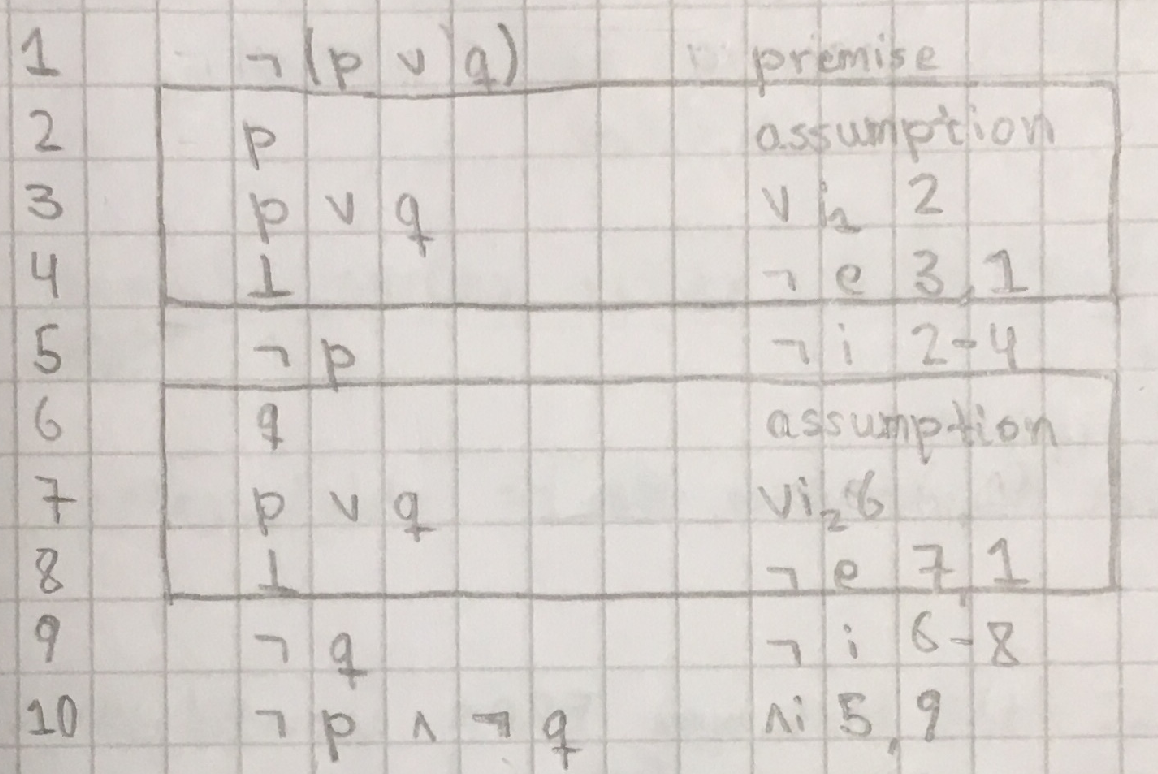
\includegraphics[scale=0.25]{de-morgan-valid}
   
   In Prolog notation, this proof is written:

\begin{verbatim}
   [1,   neg(or(p, q)),          premise],
   [
      [2,   p,                   assumption],
      [3,   or(p, q),            orint1(2)],
      [4,   cont,                negel(3, 1)]
   ],
   [5,   neg(p),                 negint(2, 4)],
   [
      [6,   q,                   assumption],
      [7,   or(p, q),            orint2(6)],
      [8,   cont,                negel(7, 1)]
   ],
   [9,   neg(q),                 negint(6, 8)],
   [10,  and(neg(p), neg(q)),    andint(5, 9)]
\end{verbatim}

   The proof verification algorithm (view appendix)
   successfully identifies this as a valid proof. To do this,
   the algorithm does the following:

   \begin{enumerate}
      \item \texttt{verify(InputFileName)} is called
            and reads in the proof from the specified file.
            The premises are stored in an array called
            \texttt{Premises}, the sequent's conclusion is
            stored in \texttt{Conclusion}, and the array
            containing the proof is stored in \texttt{Proof}.

      \item When Prolog has parsed the file, the rule
            \texttt{valid\_proof(Premises, Conclusion, Proof)}
            is invoked, which in turn calls
            \texttt{verify\_end(Conclusion, Proof)} and
            \texttt{verify\_proof(Premises, Proof, [])}, in
            the given order.

      \item \texttt{verify\_end(Conclusion, Proof)} ensures 
            that the final line of the proof is the same as
            the sequent's conclusion. This is achieved by
            first applying Prolog's built-in \texttt{last/3}
            predicate to extract the last element (line) in
            \texttt{Proof}, and then utilizing \texttt{nth0/3} 
            to select the formula present on the last line. If
            the proof is valid, this formula is equal to
            the sequent's conclusion. Accordingly, 
            \texttt{verify\_end} concludes with an equality
            check that ensures that the described equality
            holds.

      \item
         \texttt{verify\_proof(Premises, Proof, Verified)}
         recursively validates the provided proof
         line-by-line, from top to bottom. It validates each 
         line (element in \texttt{Proof}) by invoking 
         \texttt{rule/3} wite the premises, line, and 
         previously verified lines as arguments. 
         \texttt{rule/3} then returns \texttt{true} whenever 
         the line follows by natural deduction from the 
         premises and previously verified lines, and false
         otherwise. If a line is valid, it gets appended to
         the \texttt{Verified} array and \texttt{verify\_proof}
         is called again with the yet unverified lines and
         the new array of verified lines.

      \item \texttt{rule/3} takes in the array of premises, a
            line or assumption box, and the, as of then, 
            verified lines of a proof. It then ensures that
            the line or assumption box follows by natural
            deduction from the premises and previous lines of
            the proof. It does this by inspecting the last
            element of each line, which specifies the
            deduction rule that was applied to deduce the
            formula of that line, and then checking that the
            prerequisites for using the rule are fulfilled.
            To exemplify, in the above proof the first line
            invokes the premise verification rule

\begin{verbatim}
   rule(Premises, [_, Formula, premise], _) :-
      member(Formula, Premises).
\end{verbatim}
                    
            which checks that \texttt{Formula} (the formula
            on the given line) is a member of
            \texttt{Premises}. If \texttt{Formula} is a
            member, the line is valid and \texttt{rule} returns
            \texttt{true}. Line two is an assumption and thus 
            opens a box. It is handled by the assumption rule

\begin{verbatim}
rule(Premises, [[R, Formula, assumption] | T], Verified) :-
   append(Verified, [[R, Formula, assumption]], VerifiedNew),
   verify_proof(Premises, T, VerifiedNew).
\end{verbatim}

            which returns \texttt{true} if the sub-proof of the
            assumption box is valid. To verify that the
            assumption box contains a valid proof the
            assumption line is appended to the array of
            verified lines, and \texttt{verify\_proof/3} is
            called to validate the sub-proof. Within the box,
            line three is verified by ensuring that its
            application of the first disjunction introduction
            rule is valid. The below code does this

\begin{verbatim}
   rule(_, [_, or(X, _), orint1(R)], Verified) :-
      member([R, X, _], Verified).
\end{verbatim}

            by confirming that the formula $p$ has been
            deduced earlier in the proof. Line four is deduced
            by administering the rule of negation elimination.
            The below code verifies that the rule can be
            employed

\begin{verbatim}
   rule(_, [_, cont, negel(R1, R2)], Verified) :-
      member([R1, X, _], Verified),
      member([R2, neg(X), _], Verified).
\end{verbatim}

            by checking that both $p \vee q$ and 
            $\neg(p \vee q)$ occur previously in the proof
            (are members of \texttt{Verified}). When the
            sub-proof of the assumption box has been
            validated, the entire box is appended to
            \texttt{Verified} before continuing to verify the
            next line or assumption box. This ensures that no
            single line that is predicated on the assumption
            can be referenced without also referencing the
            assumption. In the above proof, the fifth line, 
            which also is the first line following the
            upper assumption box, is deduced by applying the
            rule of negation introduction. The subsequent code
            verifies that the rule can be applied

\begin{verbatim}
   rule(_, [_, neg(X), negint(R1, R2)], Verified) :-
      member([[R1, X, assumption] | T], Verified),
      last(T, BoxConclusion),
      [R2, cont, _] = BoxConclusion.
\end{verbatim}

            by establishing that the assumption box starts
            with $p$, and that it ends with a contradiction.
            \bigbreak

            Lines six through nine repeat the 
            same deductive pattern as lines two through five.
            The concluding line of the proof is arrived at by
            utilizing the rule of conjunction introduction.
            The employment of this rule is validated by the
            below code

\begin{verbatim}
   rule(_, [_, and(X, Y), andint(R1, R2)], Verified) :-
      member([R1, X, _], Verified),
      member([R2, Y, _], Verified).
\end{verbatim}

            which states that the rule can be administered if,
            and only if, both $\neg p$ and $\neg q$ occur
            previously in the proof (exist in
            \texttt{Verified}).

   \end{enumerate}

   \textbf{Invalid Proof of de Morgan's Law} \\
   The following is an invalid proof of the same sequent as
   above. Lines one through three of the proposed lines are 
   deduced by rules that we have already discussed, and hence 
   they will not be discussed any further. Nevertheless, the
   fourth and final line incorrectly applies the rule of
   negation introduction. The subsequent text examines how the
   proof verification algorithm handles this in detail.   

   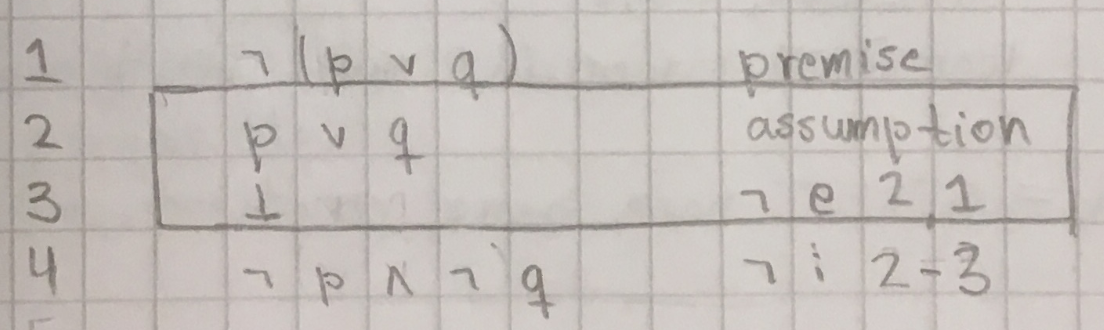
\includegraphics[scale=0.25]{de-morgan-invalid}
   
   Recall that the negation introduction rule can be employed
   to conclude $\neg \phi$, for some formula $\phi$, if, and 
   only if, there exists a box starts with an assumption of
   $\phi$ and ends in a contradiction. The proof passes the
   latter requirement, which is enforced by the code

\begin{verbatim}
   last(T, BoxConclusion),
   [R2, cont, _] = BoxConclusion.
\end{verbatim}

   but fails the former, as the assumption $\phi = p \vee q$
   combined with the contradiction and negation introduction 
   rule, can only be used to conclude $\neg (p \vee q)$, and
   not $\neg p \vee \neg q$.

\begin{table}[t]
\centering
\begin{tabular}{|l|l|l|}
   \hline
      \textbf{Predicate} 
      & \textbf{Parameters}                                  
      & \textbf{Truth Conditions} \\
   \hline
      \texttt{verify}             
      & \texttt{InputFileName}  
      & \texttt{valid\_proof} \\
   \hline
      \texttt{valid\_proof}       
      & \begin{tabular}[c]{@{}l@{}}
         \texttt{Premise} \\ 
         \texttt{Conclusion} \\ 
         \texttt{Proof}
      \end{tabular}          
      & \begin{tabular}[c]{@{}l@{}}
         \texttt{verify\_end} \\
         \texttt{verify\_proof} 
      \end{tabular} \\  
   \hline
      \texttt{verify\_end}        
      & \begin{tabular}[c]{@{}l@{}}
         \texttt{Conclusion} \\ 
         \texttt{Proof}
      \end{tabular}                    
      & Proof ends with sequent's conclusion. \\
   \hline
      \texttt{verify\_proof}      
      & \begin{tabular}[c]{@{}l@{}}
         \texttt{Premises} \\ 
         \texttt{Proof} \\ 
         \texttt{Verified}
      \end{tabular}           
      & \begin{tabular}[c]{@{}l@{}}
         The first line, and recursively all \\ 
         subsequent lines, are provable by \\ 
         natural deduction.
      \end{tabular} \\ 
   \hline
      \texttt{rule}               
      & \begin{tabular}[c]{@{}l@{}}
         \texttt{Premises} \\ 
         \texttt{Line/Box} \\ 
         \texttt{Verified}
      \end{tabular} 
      & \begin{tabular}[c]{@{}l@{}}
         If the second argument is an \\
         assumption box, \texttt{rule} is true if \\
         the sub-proof of the box is valid \\
         (i.e. if \texttt{verify\_proof} returns true \\
         when invoked with the sub-proof as \\
         its \texttt{Proof} argument).
         \\ \\
         If the second argument is a line, the \\
         conditions determining the return \\ 
         value of \texttt{rule} differ based on what \\
         deduction rule was used to arrive at \\ 
         the formula on the line. 
         \\ \\
         For lines that are \textit{premises}, the \\
         \texttt{Formula} on the line must exist in \\
         the \texttt{Premises} of the proof.
         \\ \\
         For lines that are deduced by the \\ 
         \textit{copy} rule, the copied formula must \\
         appear previously in the proof \\
         (i.e. be a member of \texttt{Verified}).
         \\ \\
         For lines with a formula $\neg \neg \phi$, that is \\
         deduced by \textit{double negation}, \\
         \textit{introduction}, the formula $\phi$ must \\
         appear previously in the proof (i.e. \\
         exist in \texttt{Verified}). 
         \\ \\
         For lines with a formula $\phi$ that is \\
         deduced by \textit{double negation} \\ 
         \textit{elimination}, the formula $\neg \neg \phi$
         must \\
         appear previously in the proof (i.e \\
         exist in \texttt{Verified}).
      \end{tabular} \\ 
   \hline
\end{tabular}
\end{table}

\begin{table}[h!]
\centering
\begin{tabular}{|l|l|l|}
   \hline
      \textbf{Predicate} 
      & \textbf{Parameters}                                  
      & \textbf{Truth Conditions} \\
   \hline
      & &
      \begin{tabular}[c]{@{}l@{}}
         For a line with a formula $\phi \wedge \psi$ that \\
         is deduced by \textit{and introduction}, the \\
         formulas $\phi$ and $\psi$ must appear \\
         previously in the proof (i.e. exist in \\
         \texttt{Verified}).
         \\ \\
         For a line with a formula $\phi$, that is \\
         deduced by \textit{first and elimination}, a \\
         formula of the form $\phi \wedge \psi$ must \\
         appear previously in the proof (i.e. \\
         exist in \texttt{Verified}).
         \\ \\
         For a line with a formula $\phi$, that is \\
         deduced by \textit{second and elimination}, \\
         a formula of the form $\psi \wedge \phi$ must \\
         appear previously in the proof (i.e. \\
         exist in \texttt{Verified}).
         \\ \\
         For a line with a formula $\phi \vee \psi$, that \\
         is deduced by \textit{first or introduction}, \\
         a formula $\phi$ must appear previously \\
         in the proof (i.e. exist in \texttt{Verified}).
         \\ \\
         For a line with a formula $\phi \vee \psi$, that \\
         is deduced by \textit{second or introduction}, \\
         a formula $\psi$ must appear previously \\
         in the proof (i.e. exist in \texttt{Verified}).
         \\ \\
         For a line with a formula $\chi$, that is \\
         deduced by \textit{or elimination}, a formula \\
         $\phi \vee \psi$, a box assuming $\phi$ and ending \\
         in $\chi$, and a box assuming $\psi$ and \\
         ending in $\chi$, must appear previously \\
         in the proof (i.e. exist in \texttt{Verified}).
         \\ \\
         For a line with a formula $\phi \rightarrow \psi$, \\
         that is deduced by \textit{implication} \\
         \textit{introduction}, a box assuming $\phi$ and \\
         concluding in $\psi$ must appear \\
         previously in the proof (i.e. exist in \\
         \texttt{Verified})
      \end{tabular} \\
   \hline
\end{tabular}
\end{table}

\begin{table}[h!]
\centering
\begin{tabular}{|l|l|l|}
   \hline
      \textbf{Predicate} 
      & \textbf{Parameters}                                  
      & \textbf{Truth Conditions} \\
   \hline
      & &
      \begin{tabular}[c]{@{}l@{}}
         For a line with a formula $\psi$ that is \\
         deduced by \textit{implication elimination} \\
         a formula $\phi$, and a box assuming $\phi$ \\
         and ending in $\psi$, must appear \\
         previously in the proof (i.e. exist in \\
         \texttt{Verified}).
         \\ \\
         For a line with a formula $\neg \phi$ that is \\
         deduced by \textit{negation introduction} a \\
         box assuming $\phi$ and concluding in $\perp$ \\
         must appear previously in the proof \\
         (i.e. exist in \texttt{Verified}).
         \\ \\
         For a line with a contradiction $\perp$ \\
         that is deduced by \textit{negation} \\
         \textit{elimination} two formulas $\phi$ and 
         $\neg \phi$ \\
         must appear previously in the proof \\
         (i.e. exist in \texttt{Verified}).
         \\ \\
         For a line with a formula $\phi$ that is \\
         deduced by \textit{contradiction} \\
         \textit{elimination} a line with a \\
         contradiction $\perp$ must appear \\
         previously in the proof (i.e. exist \\
         in \texttt{Verified}).
         \\ \\
         For a line with a formula $\neg \phi$ that is \\
         deduced by \textit{modus tollens} a formula \\
         $\phi \rightarrow \psi$, and a formula $\neg \psi$,
         must \\
         appear previously in the proof (i.e. \\
         exist in \texttt{Verified}).
         \\ \\
         For a line with a formula $\phi$ that is \\
         derived by a \textit{proof by contradiction} \\
         a box assuming $\neg \phi$ and ending in a \\
         contradiction $\perp$ must appear \\
         previously in the proof (i.e. exist in \\
         \texttt{Verified}).
         \\ \\
         By the \textit{law of the excluded middle} a \\
         line with a formula of the form 
         $\phi \vee \neg \phi$ \\
         is always valid.
      \end{tabular} \\
   \hline
\end{tabular}
\end{table}

\end{document}

